\input assets/380pre

\begin{document}
\MYTITLE{Laboratory Assignment Three \\
	Combining Imperative and Declarative Programming: \\
	Implement and Empirical Evaluation}
\MYHEADERS{}
\GROUP{Ginoza, Mulvay, Ballinger, Landgrebe, McCurdy}
\PLEDGE{}
\SUMMARY{\par
	This project is to allow us to implement a benchmarking
	framework that compares the performance of JoSQL to a hand-coded-baseline program that uses
	iteration constructs.. JoSQL is a Java library that allows
	for SQL calls to perform operations on objects. We have decided to compare the
	performance of these two data entry tools by using
	different data structures (e.g.\ \textbf{ArrayList},
		\textbf{LinkedList}, \textbf{ArrayDeque}, and \textbf{Vector}).
	\smallskip \par
	We also  decided to compare the performance of these data
	structures on different hardware. The hardware we will be comparing is a
	Dell OptiPlex 380 -- Core 2 Duo E7500 2.93 GHz with 4 GB of RAM versus a
	Mid 2011 MacBook Pro Core 2 Duo Core i7 (I7-3520M) 2.9 Ghz with 8GB of RAM.}

\begin{enumerate}
	\item \textbf{A five paragraph commentary on the work that each team member completed.}\par
		\textit{Every member of the group will individually be submitting this required
			deliverable.}
	\item \textbf{A full-featured description of the key features provided by the JoSQL library.}\par
		\begin{itemize}

			\item \textbf{Performance: }\par
				The more work you expect JoSQL to do the longer it will take to do it.
				If your WHERE clause does not significantly limit the number of objects
				that the rest of the query should work on, then obviously the rest
				of the query has more work to do, which equates to more processing time.

			\item \textbf{Query: }\par 
				This class in JoSQL allows for a developer of the Java programming language
				to apply arbitrary SQL statements to a collection of Java objects.

				\begin{center}
					\textbf{Simple Example: }\par
					Query q = new Query ();\par
					q.parse (sql);\par
					List results = q.execute (java.util.List);
				\end{center}

			\item \textbf{Where: }\par
				Allow for searching through data sets where objects---Strings
				in this lab---match what is begin searched for
				in the \textbf{Where} clause.
				\begin{center}
					\textbf{Simple Example: }\par
					WHERE  name LIKE `\%SEARCH HERE'
				\end{center}

			\item \textbf{Bind Variables: }\par
				Bind variables allow you to place ``markers'' inside the SQL 
				statement that will then be replaced at execution time with the values supplied.
				\begin{center}
					\textbf{Simple Example: }\par
					q.setVariable (``:name'', myObj)
				\end{center}
			\item \textbf{Custom Functions: }\par
				Custom functions are basically those specified by the developer
				to extend the JoSQL functionality in some way. 
				Custom functions can override the built-in functions.
				\begin{center}
					\textbf{Simple Example: }\par
					public String to\_string (Object o)
					\medskip

					\textbf{Referred to in SQL with:}\par
					SELECT to\_string (12345)\par
					FROM   java.lang.Object
				\end{center}
				\begin{flushleft}
					\textit{Note:} Custom functions are searched for in the order 
					in which their ``handler Object'' are added to the Query object.
				\end{flushleft}
				\begin{center}

					Query q = new Query ();\par
					q.addFunctionHandler (new MyFunctionHandler1 ());\par
					q.addFunctionHandler (new MyFunctionHandler2 ());
				\end{center}
			\item \textbf{Accessors:}\par
				An accessor is basically a way of accessing information held
				with an object (this is performed by using Java Reflection). The
				accessor provides a textual way of representing the public
				methods names or fields that are accessed, separated by ".".
				\begin{center}
					\textbf{Example, class java.io.File:}\par
					To access the getName method, use:
					name or getName.
				\end{center}

			\item \textbf{Save Values:}\par
				A save value is just an "identifier", usually a 
				java.lang.String(although any object can be used), that acts as
				a key for a value. The value can be any object.. Save values are
				stored in the Query object and are available to the developer
				after the query has completed. Save values are assigned either
				by a function or in the EXECUTE ON clause.

			\item \textbf{Expressions:}\par
				Expressions (modeled using the Expression object) are the basic
				"unit" within JoSQL. As such expressions can be interchanged and
				used just about everywhere (this means that even binary
					expressions such as x = y can be used in the SELECT part of the
					statement). Each expression in JoSQL must return a value, even
				if the value is null. In this way it means that comparisons
				between expressions can occur and the result of evaluating an
				expression is suitable for returning in query execution results. 
				\begin{center}
					\textbf{Various types of JoSQL
						Expressions}\par
					Binary expression - this type of expression represents the
					result of comparing a LHS with a RHS. For example 1 = 1. Just
					about all expressions that can be used in a Where clause are
					binary expressions.

					Aliased expression - this type of expression represents an
					expression that has an alias associated with it.

					Value Expression - this type of expression represents a value,
					such as a constant, a bind variable, the result of executing a
					function or even a sub-query.
				\end{center}

		\end{itemize}
	\item \textbf{The output from each team member's use of the FileFinder.java program.}\par
		\textit{These can be found after the seven posed questions.}

	\item \textbf{The properly formatted and documented version of the source code
			for your benchmarks.}\par
		\textit{These can be found after the seven posed questions and the output of our runs of FileFinder.java.}

	\item \textbf{The CSV data files resulting from all of the runs of your
			benchmarking framework.}\par
		\textit{The data files containing the results can be found after our source code.}

	\item \textbf{A comprehensive report describing our benchmarks, evaluation
			metrics, and results.}\par
		The purpose of this laboratory assignment was to compare the performance of
		JoSQL---SQL for Java Objects---to a hand-coded implementation of a search
		algorithm. We wrote four hand-coded versions of this algorithm which implement
		different data structures: the \textbf{ArrayList, ArrayDeque, LinkedList,} and \textbf{Vector}.
		We also decided to compare the hardware constraints of a
		Dell OptiPlex 380 -- Core 2 Duo E7500 2.93 GHz with 4 GB of RAM and a
		Mid 2011 MacBook Pro Core 2 Duo Core i7 (I7-3520M) 2.9 Ghz with 8GB of RAM.

		\medskip \par
		We found that JoSQL was not the fastest search algorithm. When compared with the 
		ArrayDeque, the JoSQL was up to 32 times slower than our hand-coded implemetation.

		\medskip \par
		We used differently-sized inputs to determine whether size was a factor; size did 
		not exhibit a significant difference when comparing the speed in nanoseconds of the 
		two algorithms.. In some cases the larger data set was actually searched more quickly. 
		When searching for ``medium'', the most common word in the CSV file, with the data 
		structure ArrayList, we observed that the hand-coded version completed the search in 
		760000 ns compared to the 835000 ns while searching for ``winter'', the least common word.
		Here, we can conclude that size is not significant, but in future studies we will have to 
		consider that we did not vary size as much as we could have.

		\medskip \par
		Concerning hardware constraints, the Dell ran every algorithm in less than than
		the Mac, even when controlling for confounding variables such as other open
		programs. We think the minute increase in speed per core that the Dell has may
		have allowed it to perform these tasks in fewer nanoseconds, but we acknowledge that
		this is not enough to account for the hugh variablility we observed. 

		\medskip \par
		One noticable trend was that the performance of the ArrayList, LinkedList, Vector, 
		and ArrayDeque data structures was much quicker than the JoSQL. A comparison of averages
		showed that the JoSQL was much slower than the hand-coded version.

		\begin{figure}[h!]                                                              
			\centerline{\includegraphics[scale=1]{../pic/dell.png}}                       
			\caption{Times when run on Optiplex 380}
		\end{figure}          

		\newpage
		\begin{figure}[h!]                                                              
			\centerline{\includegraphics[scale=1]{../pic/dell.png}}                       
			\caption{Times when run on MacBook Pro}
		\end{figure}          

	\item \textbf{The presentation slides to support your team's five minute
			presentation.} \par
		\textit{This will be presented in the laboratory session on September 24, 2014.}


		\newpage
		\begin{figure}[h!]                                                              
			\centerline{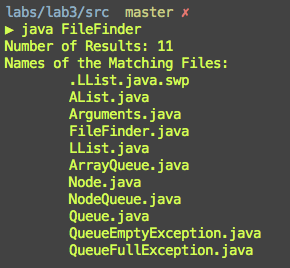
\includegraphics[scale=0.5]{../pic/colton.png}}                       
			\caption{Output of Colton's FileFinder.java}                                         
		\end{figure}          

		\begin{figure}[h!]                                                              
			\centerline{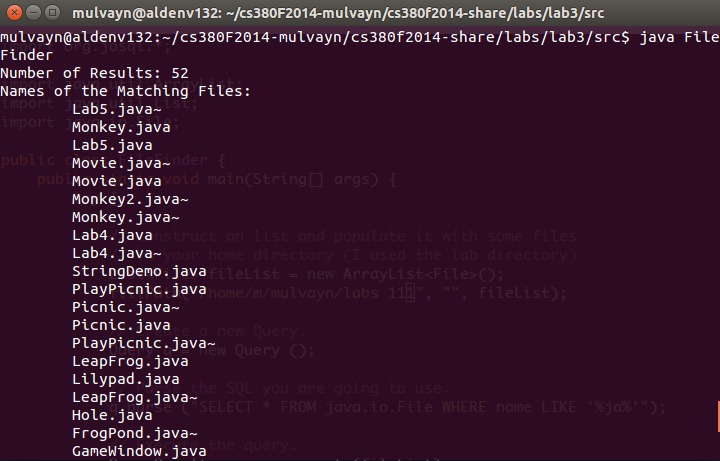
\includegraphics[scale=0.5]{../pic/Nick.png}}                       
			\caption{Output of Nick's FileFinder.java}                                         
		\end{figure}          

		\begin{figure}[h!]                                                              
			\centerline{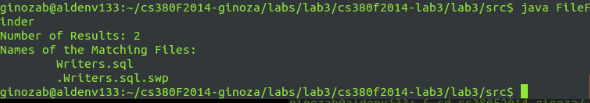
\includegraphics[scale=0.5]{../pic/Brandon.png}}                       
			\caption{Output of Brandon's FileFinder.java}                                         
		\end{figure}          

		\begin{figure}[h!]                                                              
			\centerline{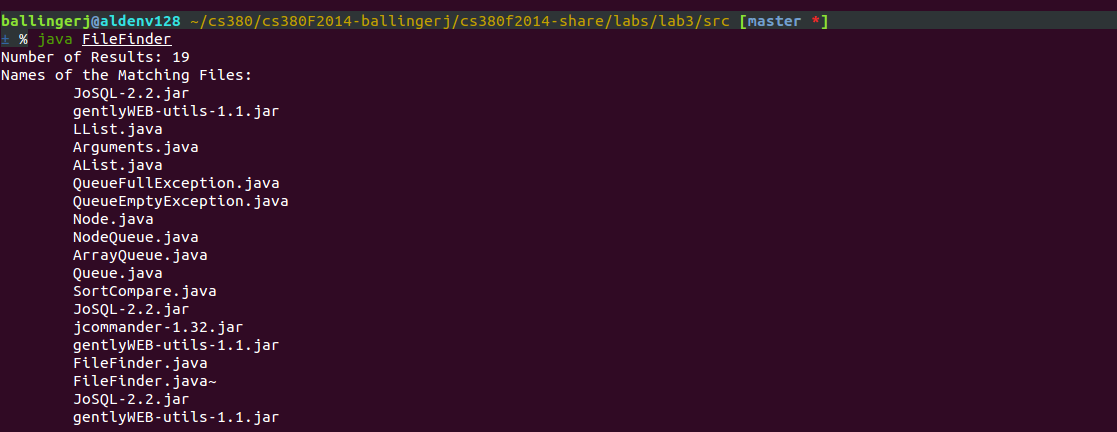
\includegraphics[scale=0.5]{../pic/Jake.png}}                       
			\caption{Output of Jake's FileFinder.java}                                         
		\end{figure}          

		\begin{figure}[h!]                                                              
			\centerline{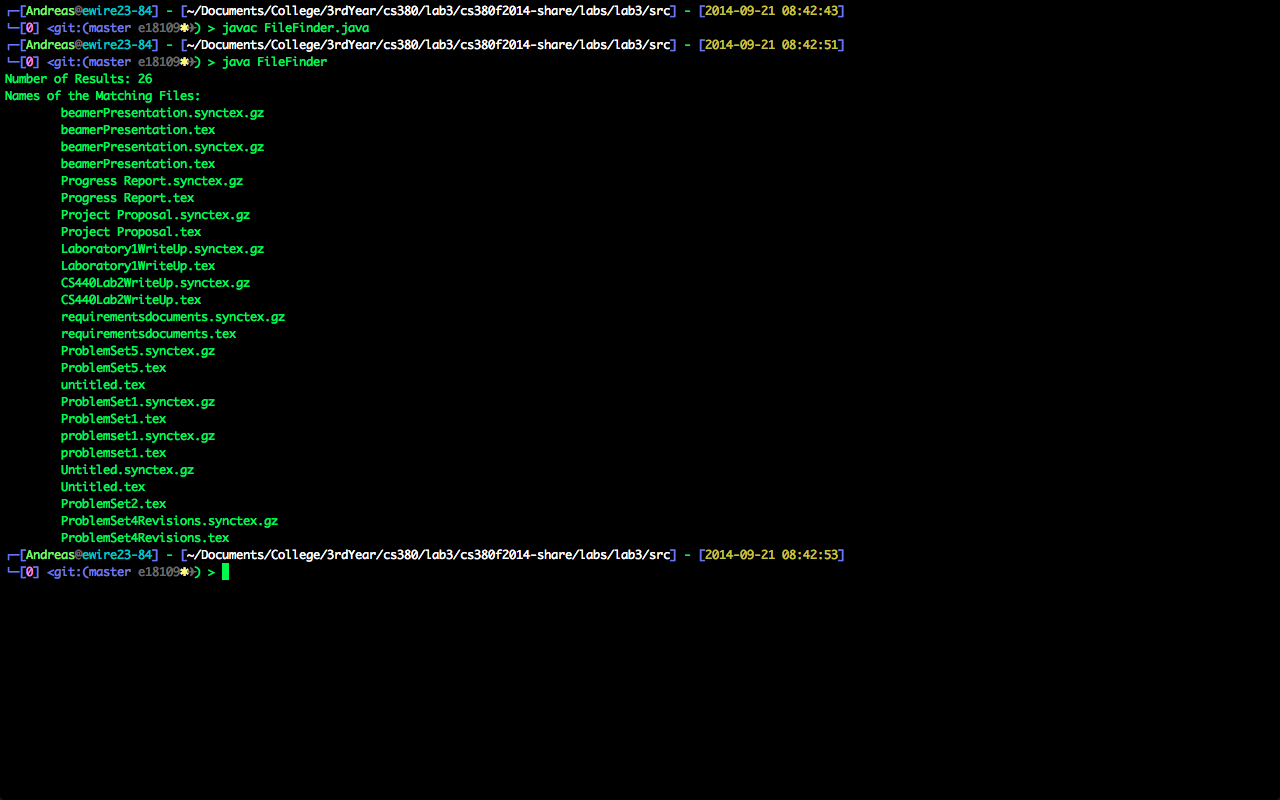
\includegraphics[scale=0.25]{../pic/Andreas.png}}                       
			\caption{Output of Andreas's FileFinder.java}                                         
		\end{figure}          
		\newpage                                                                
		\textit{The entirety of the source code for our benchmarking framework is on the following pages.}

		\vspace{5in}
		\verbatiminput{../src/AList.java} 
		\newpage                                                                
		\verbatiminput{../src/LList.java} 
		\newpage                                                                
		\verbatiminput{../src/Vect.java} 
		\newpage                                                                
		\verbatiminput{../src/ADeque.java} 
		\newpage                                                                
		\verbatiminput{../src/Arguments.java} 
		\newpage                                                                
\end{enumerate}
\end{document}
